\documentclass[class=article, crop=false, draft=true]{standalone}
\usepackage{graphicx}
\graphicspath{{../Figures}}

\usepackage{amsmath}

\usepackage{cleveref}

\begin{document}
%equations, bib. \\
\section{Previous project work}
The specialization project focused on making the framework for this thesis and for further work on the Plan Sea project in general. In this section, the results of the specialization project will be presented as it forms the basis for further work.

Originally, the goals of the specialization project were as follows:
\begin{enumerate}
\item Create a simulation to be used in later work
\item Validate the performance of the simulation
\item Create a rudimentary control system for the simulation that can be further developed later
\item Do basic research that can be implemented in this thesis
\end{enumerate}
These goals were achieved with great success. Here is a short summary of each goal and its results.

\subsection{Creating the simulation}
The simulation framework AGX Dynamics was chosen based on a recommendation from a professor based on its ability to do wire simulations well, in addition to it having both a hydrodynamic simulation package and a package that could interface with ROS2. It was considered to build a simulation from scratch, but this was deprioritized due to the amount of work this would pose.

The two vessels are simulated as simplified shapes, the surface vessel as a coarse model, while the ROV is simulated as a simple box. The simulation is mostly unchanged from the original setup, though some additional work has been done and this is further discussed in \cref{sec:simulation_work}

\subsection{Validating the simulation}
The simulation was validated by comparing the tension measured in the tether to a calculated drag force that would be expected. The surface vessel would be moving at constant speed and the ROV dragged behind. This was done at several speeds, and the tension was measured both on average and over time. The measured tension was then compared with a manually calculated drag force using the drag equation. The simulation was found to perform within \(\pm 20\%\) of the calculated drag, which given the assumptions made was concluded to be well within reasonable limits. Further discussion of this can be seen in section 4.2 of the specialization report \cite{specialization}

\subsection{Creating a control system}
A control system is a simplified abstraction of all the logic that is behind actually controlling a system. A "system" in this sense is any collection of real-world, digital, chemical or mechanical parts that accept some sort of affecting input and provide some resultant output. In this case, the movement of the vessels are the system of interest. The inputs of the system is the commands given to thrusters, cranes, or other means of moving the vessel, while the output of the system is the physical movement of the vessels and their components in space.

The control system which was created in the specialization project was implemented directly in the same script as the simulation ran on. This was not ideal, but it did work. As it was implemented, it could control both the heading of the vessel towards its waypoint as well as its total force applied. It was implemented as navigating to a list of points, changing to the next point after it reached some steady state around the current one. The movement of the ROV and crane was not controlled in the control system achieved in the specialization project.

As mentioned, the control system was not implemented in ROS2, as was the plan. This was not done due to issues with initializing a ROS workspace and decoupling the work already done. This has been achieved in this project however, and is further discussed in \cref{sec:simulation_work}.

\subsection{Basic research}

\section{State of the Art}
\subsection{Physical issues}
\subsection{Simulation issues}

\section{Mathematical basis}


\section{Modelling and Control Design}

\begin{figure}
    \centering
    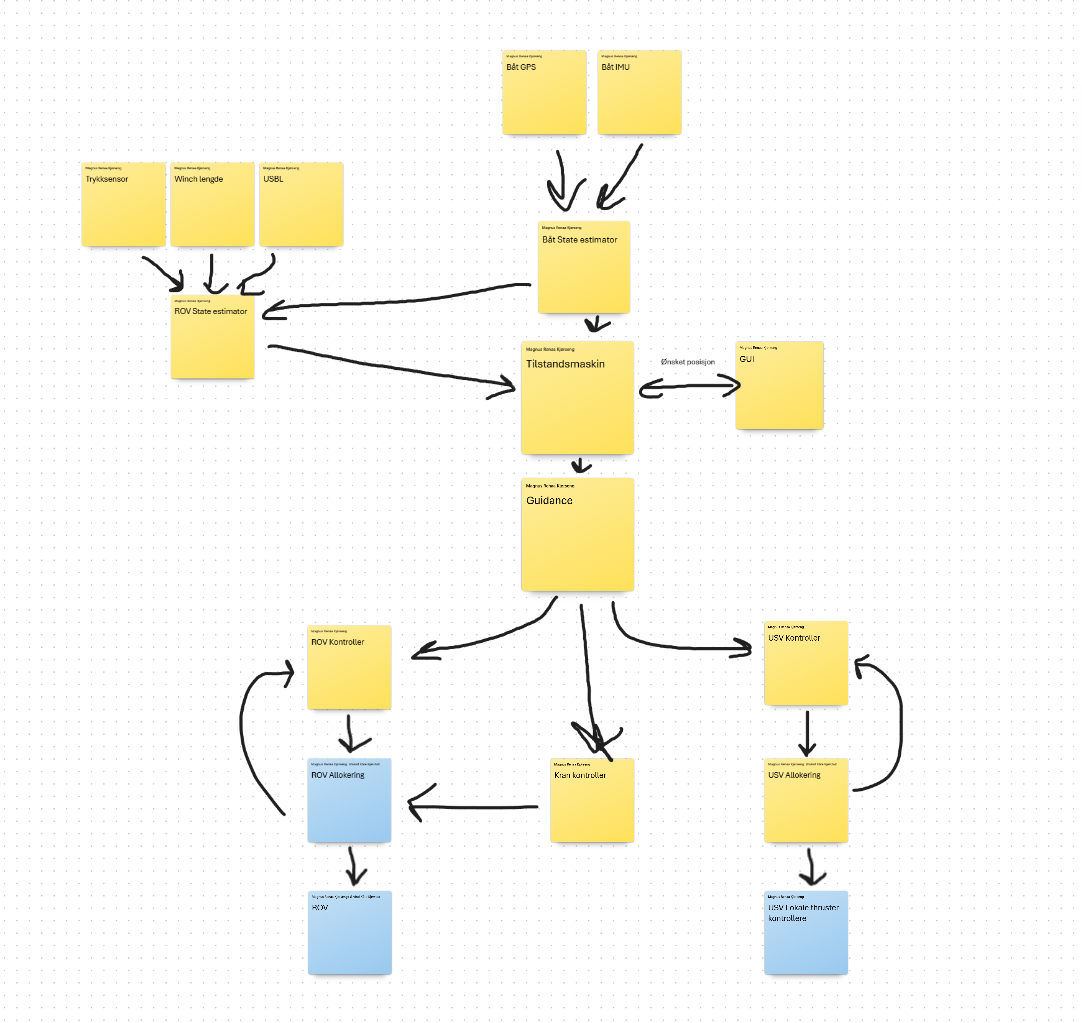
\includegraphics[width=0.9\textwidth]{control-system}
    \caption{A sketch of the control system design. TODO: Fiks bedre illustrasjon}
    \label{fig:control-system}
\end{figure}

\section{Sensorics}
The first step to knowing where to go is knowing where you are.

There are several pieces of sensorics that will be used for positioning of the system.

\subsection{GNSS}
Firstly, Global Navigational Satellite Systems, or GNSS, will be used to position the USV. There are several separate systems for GNSS, including GPS, Gallileo and GLONASS to mention a few.

The exact workings of how GNSS works is not essential for this project. The important part is that GNSS requires a clear view of the sky and allows for accuracies of approximately 2m. While this accuracy would be usable for this project, a higher accuracy would be preferable. Luckily, there exist systems that allow for this greater accuracy as well. For this project, an RTK enabled GNSS reciever has been acquired. RTK uses a secondary base station and direcct communication between the receiver and the base station to produce highly accurate readings, on the order of millimeters or centimeters, as opposed to meters.

GNSS requires a clear view of the sky, this means that it's not usable indoors to a large extent, and it's also not usable under water. Water is an excellent absorber of the entire spectrum of electromagnetic radiation, from radio all the way to gamma rays. This means that separate positioning is required for positioning the ROV.

NMEA-0183 GGA message used for recieving position

\subsection{USBL}
The main method for positioning the ROV will be through an ultra-short baseline system, USBL. USBL works sonically by having a tranciever on the surface vessel which transmits a sound signal, the signal is picked up by a transponder under water which transmits a response signal. The tranciever through an array of hydrophones picks up the response and is able to find the direction it came from as well as the distance. Direction comes from differential time of response for the different hydrophones, while distance comes from a combination of time-of-flight and doppler (TODO: sjekk om doppler faktisk er en greie her).

TODO: Legg inn figur av USBL

Available and accurate

Need to consider limitations of accuracy of USBL re: salinity, water temperature/density, etc.

\subsection{IMUs}
Both the surface vessel and the ROV will have inertial monitoring units, IMUs, installed. These detect changes in velocity and acceleration in 6dof, allowing for relative position to be found. IMUs are most useful as a dead-reckoning tool, i.e. using a last known location and a set of velocities/directions, an approximate current position can be found.

For this solution, the IMUs will be used as supplemental data to the USBL and GNSS systems. This is to allow for a more complete model of the movement of each of the vessels. Especially for the surface vessel, things like heave from waves is not necessarily easy to get from GNSS data, but will be trivial to find from an IMU. Using this it's also possible to potentially build a model of the current seastate which allows for better predictive DP rather than just a reactive system which is what's currently implemented.

\subsection{ROV Depth measuring devices}
The ROV will have a couple of extra sensors for finding depth and distance from the seafloor.

A pressure sensor is able to fairly accurately (within 1m) tell the depth of the ROV. Pressure sensors can work in many ways, the ones available here use a two chamber differential approach with a flexible membrane between two chambers. One chamber is open to the atmosphere and the other is closed off with a known pressure inside. By measuring the amount the flexible membrane stretches, it is possible to find the pressure differential between the two chambers. Knowing this differential and the calibration pressure, it's possible to estimate the depth by using the knowledge that water pressure increases by approximately 10kPa per meter of depth. More accurate values can be found but depend on things like water temperature, salinity and others.

Another tool which will give an upper bound to the depth of the ROV is the length of wire which has been payed out. Due to effects because of lag and currents as mentioned previously (TODO: faktisk skrive dette) the length of the wire will in most cases be greater than the actual depth of the ROV or the distance to the ROV. It can still be useful to know this length though, both as an absolute upper bound to fact-check the other sensors, but also to keep track of how much of the wire remains and how the winding system may work.

Additionally, the ROV will be mounted with a laser based time-of-flight sensor. This sensor works similarly to the USBL system mentioned above but using laser light instead of sound. A laser is sent from the sensor, hits obstacles or the seafloor and bounces back. The light bouncing back is detected by the sensor and doing time-of-flight calculations, it's possible to find the distance from the sensor to the object in question. This can be done to very accurately measure the distance to objects or the seafloor to avoid collisions or aid in picking them up.

Another example of something that could potentially help is taut wire positioning. Taut wire positioning works by having a wire anchored at a given point and then measuring the angle at which the wire exits a boom or whatever is holding it in place. By knowing the length of wire, the fact that the wire is taut, and the angle at which the wire is extending from the surface vessel, it is possible to find a relative position between the surface vessel and the anchor. It is possible that with a very heavy ROV, or if the ROV picks up a large load, that taut-wire might work for positioning, but given the effects on the wire seen in simulation it's very probable that taut-wire will provide more trash data than useful. Due to this it's disregarded as an option.


\section{State estimation}
The state estimator takes in the various sensor data and builds a single model of position. This is done because different sensors might have different accuracies or update times. The state estimator handles these discrepancies and builds a cohesive model. The state estimator feeds this more accurate position into the guidance system (TODO: Spørre øivind om det er guidance eller state machine som får posijonen. State machine skal jo bare være et informasjonslager?)

\section{State machine}
The state machine keeps track of variables for the total control system. These include current position, but also things like desired position or operating mode, gathered from the GUI.

\section{GUI}
The GUI is where a human operator interfaces with the control system. The GUI is supposed to include a position input for the surface vessel, mode switching between USV-Master, ROV-Master and idle/standby modes, along with other functions.

\section{Guidance}
The guidance system provides finer control of the vessel than what would be achieved by a state machine and controller alone. For instance it smooths acceleration/deceleration of the vessels by providing imaginary set points between the current position and the actual set point.

\section{Controller}
The controller finds a desired force input based on the difference (error) between the current position and the desired position. The current implementation uses a simple PID for this. This force input is fed forward to the allocator.

The shape of the force coming out of the controller is as \[\tau = \begin{bmatrix}X \\ Y \\ N\end{bmatrix}\]

\section{Allocation}
The allocator works like a translation layer between the controller and the local controllers. The controller provides a force input on the vessel's center of gravity. By inputting forces on the center of gravity, no torques are produced from lateral forces, nor lateral forces from the torque.

In abstract terms, the allocator finds and applies a transformation matrix \(T\) such that \[Tf = \tau\] where \(f\) is a vector of vectors with the lateral forces for each thruster. For this case with two thrusters, it will look something like \[f = \begin{bmatrix}x_1 \\ y_1 \\ x_2 \\ y_2 \end{bmatrix}\]
The transformation matrix can be written explicitly for the USV, since it has a very simple thrust configuration. For larger configurations it might be better to write each thruster's transformation individually and either add or remove them depending on the type of move necessary (larger moves use only larger thrusters etc.).
\begin{equation}\label{eq:transform_matrix}
T = \begin{bmatrix}1 & 0 & 1 & 0 \\ 0 & 1 & 0 & 1 \\ -l_{y_1} & l_{x_1} & -l_{y_2} & l_{x_2}\end{bmatrix}
\end{equation}

\begin{figure}
    \centering
    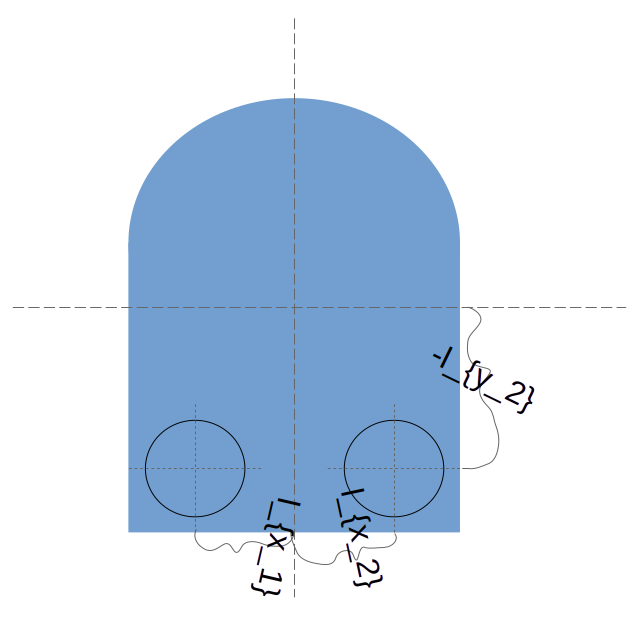
\includegraphics[width=0.9\textwidth]{thruster_position_sketch}
    \caption{Sketch of how the thruster position values in \cref{eq:transform_matrix} are found. The thruster configuration will be input to the allocator through a config file.}
    \label{fig:thruster_position_sketch}
\end{figure}

Since \(\tau\) and \(T\) are known, we can find \(f\) by performing a pseudoinverse on \(T\) leading us to the equation

\begin{equation}\label{eq:final_allocator}
f = T^\dagger \tau
\end{equation}

where \(T^\dagger\) is the pseudoinverse of \(T\).

This can also be written longform as

\begin{equation}\label{eq:long_allocator}
\begin{bmatrix}x_1 \\ y_1 \\ x_2 \\ y_2 \end{bmatrix} = T^\dagger \begin{bmatrix}X \\ Y \\ N\end{bmatrix}
\end{equation}

The full matrix for \(T^\dagger\) is omitted because the pseudoinverse of a non-square matrix tends to be large and ugly. It will only be handled by machine hands anyway, and as such doesn't matter right now.

The ROV has a built-in allocator which works well enough. The only issue with the ROV's allocator is that it's configured for a neutrally buoyant vessel. For this system we need to filter the vertical force component so the ROV only handles high-frequent/small-amplitude responses and the crane handles larger amplitudes and lower frequencies. This is also necessary because of elasticity in the lifting cable.

\section{Local control and physical response}
The vessel in this iteration has two thrusters. The ROV has a closed working solution and will not be considered here except for in the hypothetical. Each of these local controllers receive a two-component vector (or three-component in the case of the ROV) which instructs the controller what the desired thrust is. The azimuth thrusters on the USV are able to apply a force in one direction (parallel to the propeller axis), but they are able to vector this one-dimensional thrust using the azimuth ring.

\end{document}
